\documentclass{article}
\usepackage{CJKutf8}
\usepackage{multirow}
\usepackage[cmex10]{amsmath}
\usepackage{listings}
\usepackage{algorithmic}
\usepackage{algorithm}
\usepackage{epsfig}
\usepackage{amsopn}
\usepackage{subfigure}
\usepackage{cite}
\usepackage{courier}
\makeatletter
\makeatother
\begin{CJK}{UTF8}{gbsn}
\usepackage[framed,autolinebreaks,useliterate]{mcode}

\usepackage{graphicx}
\begin{document}
\title{通信与网络\\第三次编程作业}
\author{王亭午,2012011018,无210班}
\date{2015年11月30号}
\maketitle
\section{基带波形}
产生一个长为1000的二进制随机序列,0的概率为0.8,1的概率为0.2;
\subsection{问题1}对上述数据进行归零AMI编码,脉冲宽度为符号宽度的50\%对应的波形(同时给出前20位信源序列)\\
答案:可以看到,我们的代码完成了对应的编码设计,脉冲宽度保持为50\%。代码如下:
\begin{lstlisting}
N = 1001;   % sample 1000 points, 1 is added as the initial source
T = 1;  % the time period is 1 s
sampleRate = 8;

pobability = rand(1,N);
source = zeros(1,N);

source(pobability>0.8) = 1;  % generate the source
source(1) = 1;

t = 0: 1/sampleRate/N: T - 1/sampleRate/N;

% The AMI results
f = zeros(1, N);
AMI = zeros(1, N * sampleRate);

for k = 2 : 1: 1000
    f(k) = mod((f(k-1) + source(k)), 2);  % generate the f
end
send = zeros(1, N);
for k = 1 : 1: N
    if(source(k)==0)
        send(k) = 0;
    elseif(f(k) == 1)
        send(k) = 1;
    else
        send(k) = -1;
    end
    AMI((k - 1) * sampleRate + 2 : k * sampleRate - 3) = send(k);
end
\end{lstlisting}
\begin{figure}[!htb]
\begin{center}
		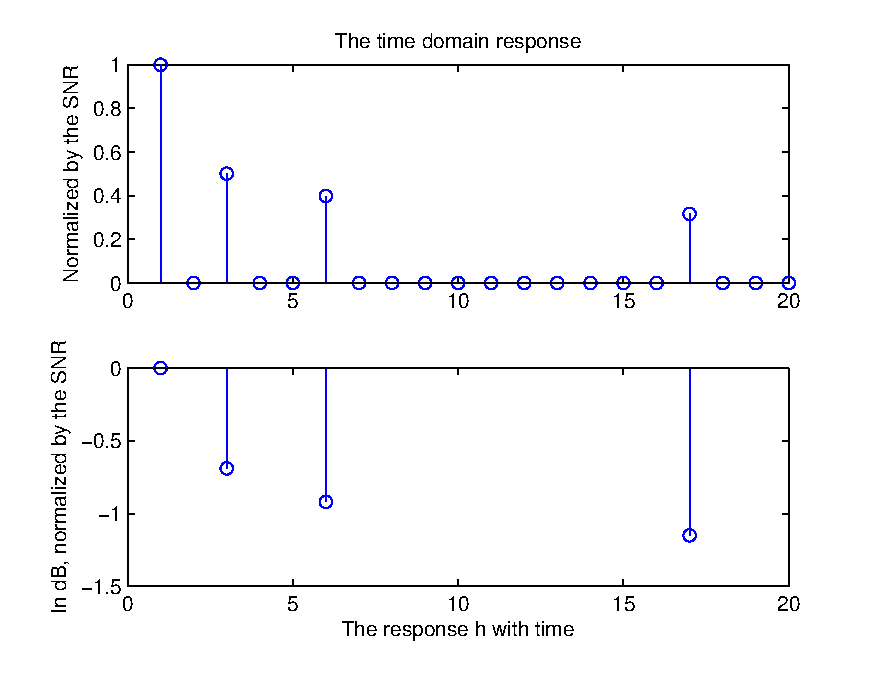
\includegraphics[width=0.8\linewidth]{1.eps}
		\caption{原始信号,和AMI编码后}
\end{center}
\end{figure}
\subsection{问题2}改用HDB3码,画出前20个符号对应的波形\\
答案:可以看到,我们的HDB3码通过使用违反规则的非法4bit串来表示4个0。代码如下:
\begin{lstlisting}
% The HDB3 code
zeroCounter = 0; odd_evenCounter=0;
HDB3 = zeros(1, sampleRate * N);
for k = 1 : 1: N
    if (source(k) == 0)
        if(zeroCounter == 3)  % now we have 3 zeros in a row
            send(k) = 1 - 2 * odd_evenCounter;
            zeroCounter = 0;
        else
            zeroCounter = zeroCounter + 1;
        end
    elseif(odd_evenCounter == 1)
        send(k) = 1;
        odd_evenCounter = 1 - odd_evenCounter;
        zeroCounter = 0;
    else
        send(k)= -1;
        odd_evenCounter= 1 - odd_evenCounter;
        zeroCounter = 0;
    end
    HDB3((k-1) * sampleRate + 3 : k * sampleRate - 2) = send(k);
end
\end{lstlisting}
\begin{figure}[!htb]
\begin{center}
		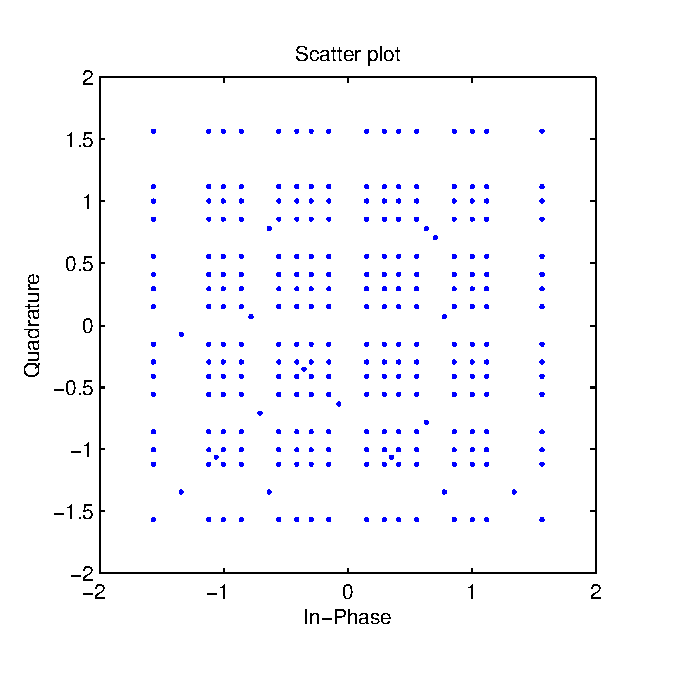
\includegraphics[width=0.8\linewidth]{3.eps}
		\caption{AMI信号,和HDB3编码后}
\end{center}
\end{figure}
\subsection{问题3}改用密勒码,画出前20个符号对应的波形
答案:同理,代码如下:
\begin{lstlisting}
% The mile code
mile = zeros(1, sampleRate * N);
send = zeros(2, N); send(2, 1) = 1;  % now the code is doubled
mile(1 : 4) = 0; mile(5 : 8) = 1;
for k = 2 :1 : N
    if(source(k)==1)
        send(1, k) = send(2, k - 1);
        send(2, k) = -send(2, k - 1);
    elseif(source(k - 1) == 1)
        send(1, k) = send(2, k - 1);
        send(2, k) = send(2, k - 1);
    else
        send(1, k) = -send(2, k - 1);
        send(2, k) = -send(2, k - 1);
    end
    % the code should be then resample to 8 times
    mile((k - 1) * 8 + 1 : (k - 1) * 8 + 4) = send(1, k);
    mile((k - 1) * 8 + 5 :(k) * 8) = send(2, k);
end
\end{lstlisting}
\begin{figure}[!htb]
\begin{center}
		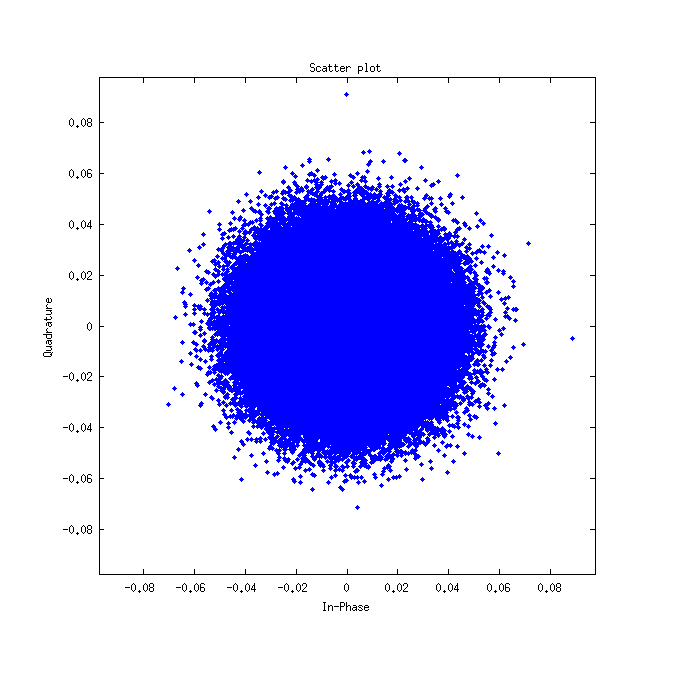
\includegraphics[width=0.8\linewidth]{4.eps}
		\caption{原始信号,和MILE编码后}
\end{center}
\end{figure}
\subsection{问题4}分别对上述1000个符号的波形进行功率谱估计,画出功率谱\\
答案:可以看到Fig. 4,我们的mile码的能量是最为集中的,不过也是最为耗能的,AMI码最不耗能。HDB3码在AMI码上加了000V和B00V脉冲,因此更加耗能。
\begin{figure}[!htb]
\begin{center}
		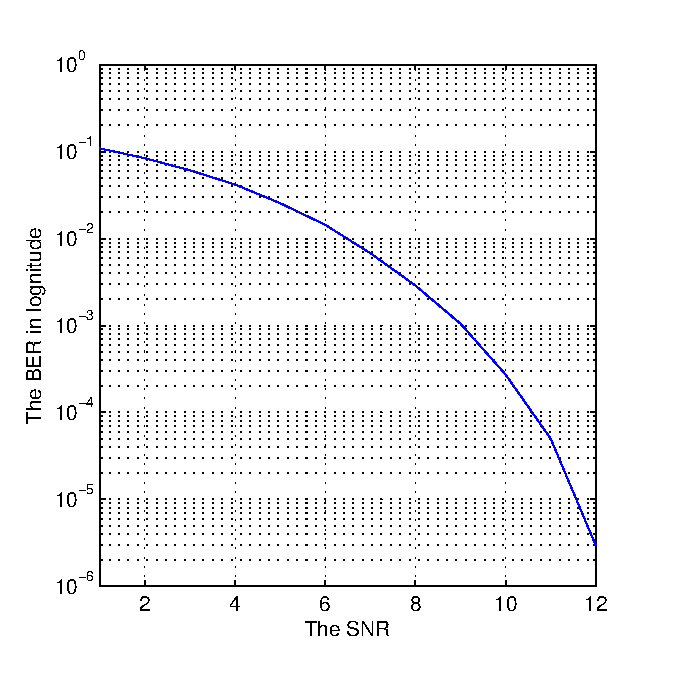
\includegraphics[width=0.8\linewidth]{5.eps}
		\caption{三个传输方式的功率谱估计}
\end{center}
\end{figure}
\subsection{问题5}改变信源0的概率,观察AMI码的功率谱变化情况\\
答案:随着概率的减小,功率谱越来越集中。可以看到,当0的概率为1的时候,功率谱理论是0,是一个连续的极小的谱,这是精度误差的原因。
当1的概率为1的时候,这个时候变成离散谱,和我们的理论期望相符合。
\begin{figure}[!htb]
\begin{center}
		\includegraphics[width=0.8\linewidth]{8.eps}
		\caption{改变0的概率,查看功率谱的变化规律}
\end{center}
\end{figure}
\section{载波波形}
产生长度为100的随机二进制序列
\subsection{问题1}发送载波频率为10倍比特率,画出过采样率为100倍符号率的BPSK调制波形(前10个比特),及其功率谱\\
答案:结果如下,分别是Fig. 6, Fig. 7,代码如下:
\begin{lstlisting}
overSampleRate = 100;
T = 1;
N = 100;
sampleRate = N * overSampleRate;

sourceGen = rand(1, N);
source = zeros(1, N);
source(sourceGen > 0.5) = 1;

t = 0: 1 / (N * overSampleRate) : T - 1 / (N * overSampleRate);
sendOrigin = zeros(1, N * overSampleRate);

for i = 1: 1: N
    sendOrigin(1 + (i - 1) * overSampleRate: i * overSampleRate) = ...
        2 * source(i) - 1;
end

f = N * 10;  % the carrier frequency
phi_0 = 0;
send = sendOrigin .* cos(2 * pi * f * t + phi_0);  % the bpsk modulation
\end{lstlisting}
\begin{figure}[!h]
\begin{center}
		\includegraphics[width=0.8\linewidth]{2_1.eps}
		\caption{前10个bit的原信号和BPSK信号}
\end{center}
\end{figure}
\begin{figure}[!h]
\begin{center}
		\includegraphics[width=0.8\linewidth]{2_2.eps}
		\caption{发射信号功率谱}
\end{center}
\end{figure}
\subsection{问题2}相干解调时假设收发频率相位相同,画出x(t)的波形,假设低通滤波器的冲激响应为连续10个1(其余为0),或连续12个1(其余为0),分别画出两种滤波器下的y(t),及判决输出(前10个比特)\\
答案:代码如下,Fig. 8, 9, 10为结果图。
可以看见,使用10个1的滤波器效果比使用12个的效果更加好,这可能是和相干时间有关的。两者的decode结果都是一样的好。
\begin{lstlisting}
% demodulation begins
x = send .* cos(2 * pi * f * t + phi_0);
lpf_1 = zeros(1, length(x)); lpf_1(1: 10) = 1;  % two low pass filter
lpf_2 = zeros(1, length(x)); lpf_2(1: 12) = 1;
figure
plot(x(1: 20 * overSampleRate))
title('The received x')
y1 = conv(x, lpf_1);
y1 = y1(1:length(x));
y2 = conv(x, lpf_2);
y2 = y2(1:length(x));
\end{lstlisting}
\begin{lstlisting}
figure
subplot(3,1,1); plot((1 + sign(y1(1: 10 * overSampleRate))) / 2);
ylim([-1.5 1.5]); title('Decoded from y1')
subplot(3,1,2); plot((1 + sign(y2(1: 10 * overSampleRate))) / 2);
ylim([-1.5 1.5]); title('Decoded from y2')
subplot(3,1,3); plot((1 + sign(sendOrigin(1: 10 * overSampleRate))) / 2);
ylim([-1.5 1.5]); title('original')
\end{lstlisting}
\begin{figure}[!h]
\begin{center}
		\includegraphics[width=0.8\linewidth]{2_3_x.eps}
		\caption{接受到的x(t)波形}
\end{center}
\end{figure}
\begin{figure}[!h]
\begin{center}
		\includegraphics[width=0.8\linewidth]{2_3.eps}
		\caption{两种滤波器下的的y(t)波形}
\end{center}
\end{figure}
\begin{figure}[!h]
\begin{center}
		\includegraphics[width=0.8\linewidth]{2_4.eps}
		\caption{问题2:判决输出}
\end{center}
\end{figure}
\subsection{问题3}接收载波频率为10.05倍比特率,初相位相同,画出x(t)的波形,假设低通滤波器的冲激响应为连续10个1,画出两种滤波器下的y(t),及判决输出(前20个比特)\\
答案:和上一问代码一样,结果如下,在Fig. 11中。虽然输出波形变得比较乱,但是结果还是对的。
\begin{figure}[!h]
\begin{center}
		\includegraphics[width=0.8\linewidth]{2_5.eps}
		\caption{问题3:判决输出}
\end{center}
\end{figure}
\newpage
\subsection{问题4}采用DPSK及延时差分相干解调,载波频率为10倍比特率,画出a, b, c, d点的波形(前10个比特)\\
答案:代码如下,我们按照课件中的流程使用延时差分想干调制解调。可以看到,我们的结果是正确的。
\begin{lstlisting}
overSampleRate = 100;
T = 1;
N = 100;
sampleRate = N * overSampleRate;

sourceGen = rand(1, N);
source = zeros(1, N);
source(sourceGen > 0.5) = 1;

t = 0: 1 / (N * overSampleRate) : T - 1 / (N * overSampleRate);
sendOrigin = zeros(1, N * overSampleRate);

for i = 1: 1: N
    sendOrigin(1 + (i - 1) * overSampleRate: i * overSampleRate) = ...
        2 * source(i) - 1;
end

f = N * 10.05;  % the carrier frequency
phi_0 = 0;
send = sendOrigin .* cos(2 * pi * f * t + phi_0);  % the bpsk modulation

% demodulation begins
x = send .* cos(2 * pi * f * t + phi_0);
lpf_1 = zeros(1, length(x)); lpf_1(1: 10) = 1;  % two low pass filter

figure
subplot(2,1,1)
plot(x(1: 20 * overSampleRate))
title('The received x')

y1 = conv(x, lpf_1);
y1 = y1(1:length(x));

subplot(2,1,2)
plot(y1(1: 20 * overSampleRate))

figure
subplot(2,1,1); plot((1 + sign(y1(1: 10 * overSampleRate))) / 2);
ylim([-0 1.5]); title('Decoded from y1')
subplot(2,1,2); plot((1 + sign(sendOrigin(1: 10 * overSampleRate))) / 2);
ylim([-0 1.5]); title('original')
\end{lstlisting}
\begin{figure}[!h]
\begin{center}
		\includegraphics[width=1.0\linewidth]{2_6.eps}
		\caption{问题4:DPSK原码,a波形,b波形,c波形,d波形和结果图}
\end{center}
\end{figure}
\subsection{问题5}DPSK及延时差分相干解调,载波频率为10.25倍比特率时,画出a, b, c, d点的波形(前10个比特)\\
答案:这个时候,我们注意到DPSK要求延时(即符号周期Ts)中有整数个载波周期,如果不满足,则应将信号变频至满足条件。
如果我们直接修改频率,会得到以下的结果Fig. 13。结果是错误的,因此我们对发射信号进行变频,代码如下:
\begin{lstlisting}
% -------------------------- frequency conversion ----------------------- %
sendFrequencyConversion = zeros(1, N * overSampleRate);
FrequencyConversion = resample(sendOrigin, 1000, 100 * Coff);
sendFrequencyConversion(1: length(FrequencyConversion)) = ...
    FrequencyConversion(:);
\end{lstlisting}
结果中,我们再把信号重新变回来,如下,结果在Fig. 14中,这个结果就是正确的了。
\begin{lstlisting}
lpf_1 = zeros(1, length(send_c)); lpf_1(1: 10) = 1;
y1 = conv(send_c, lpf_1);
y1 = resample(y1, 100 * Coff, 1000);
\end{lstlisting}
\begin{figure}[!h]
\begin{center}
		\includegraphics[width=1.0\linewidth]{2_7_0.eps}
		\caption{问题5:如果不满足延时(即符号周期Ts)中有整数个载波周期。DPSK原码,a波形,b波形,c波形,d波形和结果图}
\end{center}
\end{figure}
\begin{figure}[!h]
\begin{center}
		\includegraphics[width=1.0\linewidth]{2_7.eps}
		\caption{问题5:满足延时(即符号周期Ts)中有整数个载波周期。DPSK原码,a波形,b波形,c波形,d波形和结果图}
\end{center}
\end{figure}
\subsection{问题6}DPSK及延时差分相干解调,载波频率为10.5倍比特率时,画出a, b, c, d点的波形(前10个比特)\\
答案:同理,我们进行变频,结果如下,在Fig. 15中。
\begin{figure}[!h]
\begin{center}
		\includegraphics[width=1.0\linewidth]{2_8.eps}
		\caption{问题6:满足延时(即符号周期Ts)中有整数个载波周期。DPSK原码,a波形,b波形,c波形,d波形和结果图}
\end{center}
\end{figure}
\end{CJK}
\end{document}













\begin{equation}
f_s \geq 2(f_H - f_L) (1 + \frac{M}{N})=2(15 - 10) (1 + \frac{0}{N}) = 10\mbox{kHz}
\end{equation}
\section{任务二}
如果采样后先进行均匀量化再存贮,希望保证无量化过载的情况下量化后信噪比达到30dB,最少需要多少位量化? \\
答案:我们先求我们的信号最大最小幅度。
\begin{equation}
P = \int_{-A}^Ap(x)x^2dx = \int_{-A}^A\frac{1}{2A}x^2dx = \frac{A^2}{3} = 1
\end{equation}
得到我们的信号幅度\(A = \sqrt{3}\)。我们考虑到接受信号是白噪声,于是假设\(D = 1\)。
\begin{equation}
\begin{aligned}
SNR & = 10lg\left(\frac{S}{\sigma_q^2}\right)\\
	& = 4.77 + 20lg\left(1\right) + 6.02n \geq 30 \\
\Rightarrow \quad & n \geq 5
\end{aligned}
\end{equation}
\section{任务三}
如果要求最终分离出来的两个实带通信号信噪比均至少达到30dB,需要多少位量化?\\
答案:这个时候我们我们只需把(3)式中S=1换成\(S=10^{-6}\)。这个时候代入(1)得到结果为15。
\section{任务四}
理论计算,并编程仿真,画出原始波形,采样波形,采样频谱,重构波形,重构频谱;采样量化重构后的波形及频谱,重构误差波形及频谱。\\
答案:我们的结果图如下。
(1)可以看到,采样波形根据我们的生产规则,在12-15kHz处值比较大,在10-11kHz处值比较小,其余地方没有值。这是符合我们的期望的。\\
(2)而经过量化之后,频谱各个地方都出现了毛刺,这是我们量化误差导致的频谱上的变化。\\
(3)当我们使用n=5的量化时,12-15kHz的频谱已经可以很好的保证误差在范围内,但是10-11kHz还是没法保证。\\
(3)当我们使用n=15的量化时,所有的频谱已经可以很好的保证误差在范围内。\\
\begin{figure}[!htb]
\begin{center}
		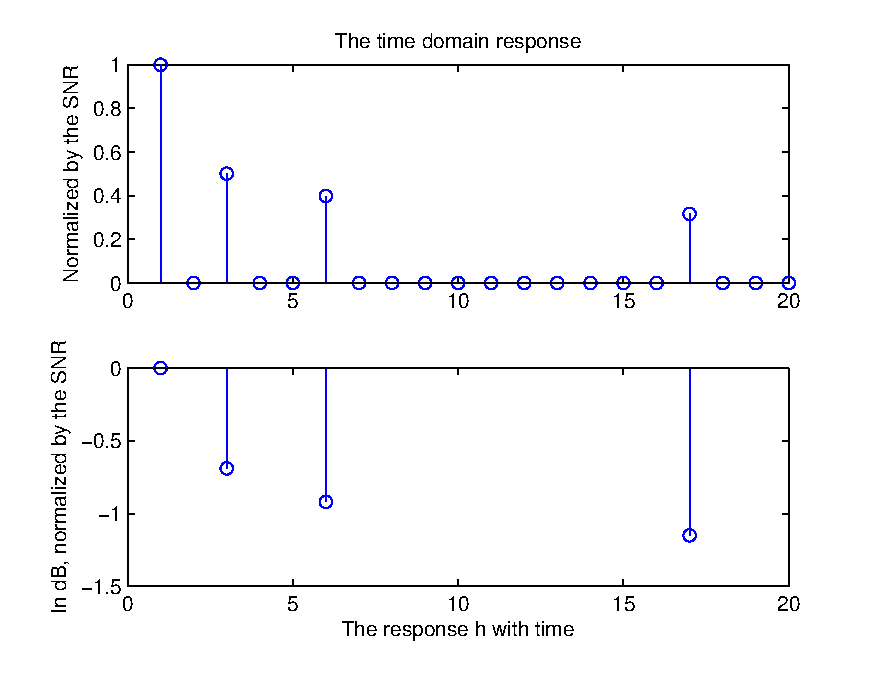
\includegraphics[width=0.8\linewidth]{1.eps}
		\caption{原始波形图}
\end{center}
\end{figure}
\begin{figure}[!h]
\begin{center}
		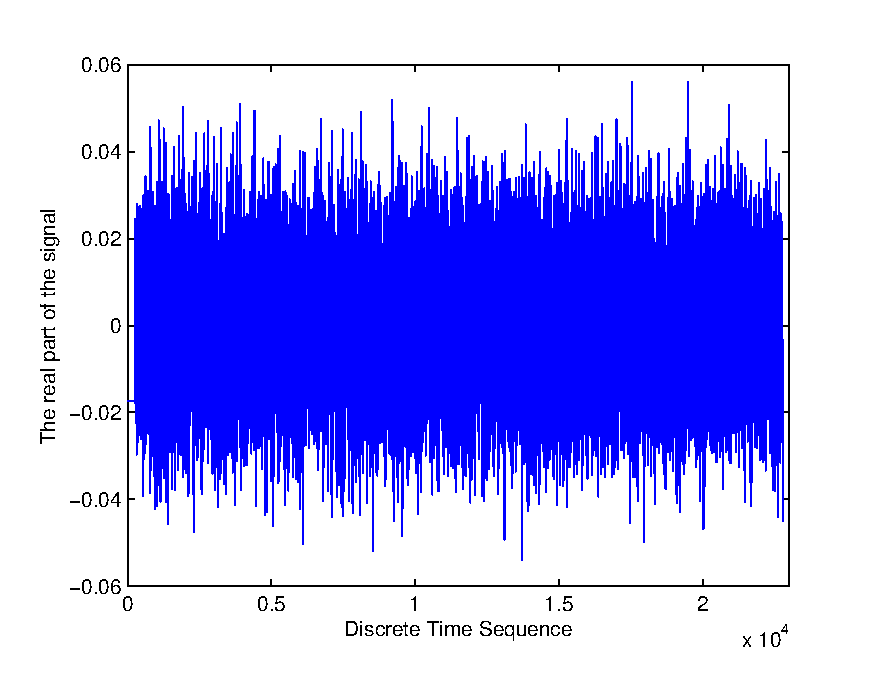
\includegraphics[width=0.8\linewidth]{2.eps}
		\caption{采样波形,采样频谱}
\end{center}
\end{figure}
\begin{figure}[!h]
\begin{center}
		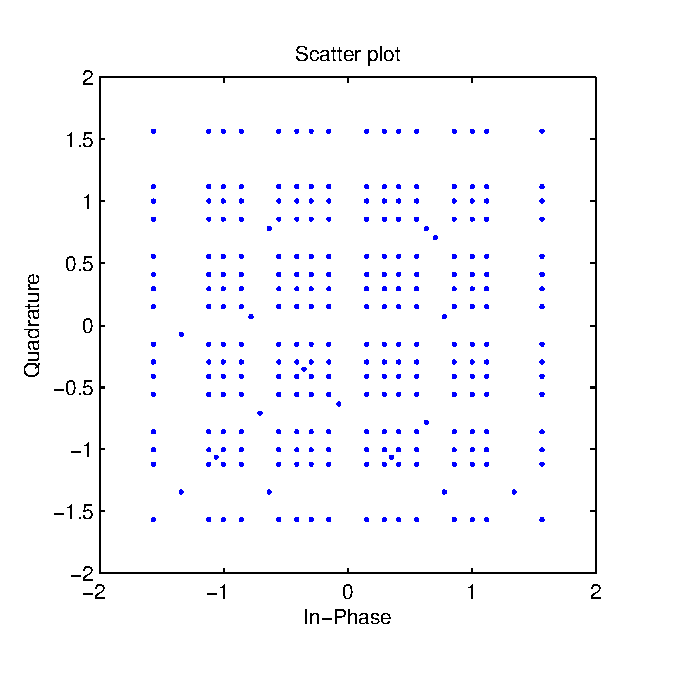
\includegraphics[width=0.8\linewidth]{3.eps}
		\caption{重构波形,重构频谱}
\end{center}
\end{figure}
\begin{figure}[!h]
\begin{center}
		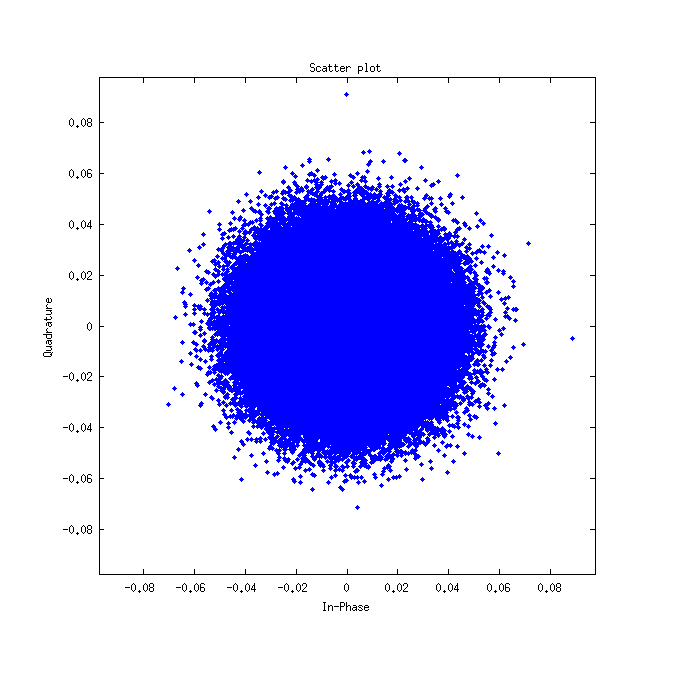
\includegraphics[width=0.8\linewidth]{4.eps}
		\caption{采样量化重构后的波形及频谱}
\end{center}
\end{figure}
\begin{figure}[!h]
\begin{center}
		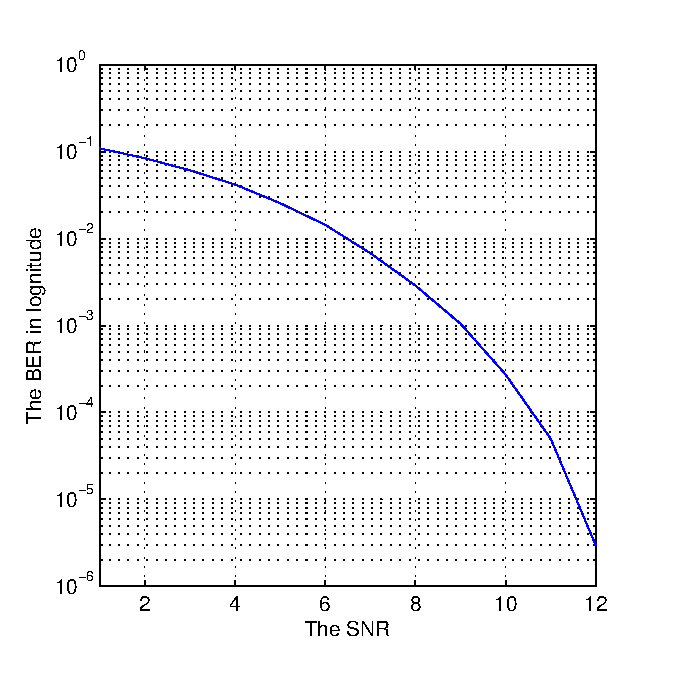
\includegraphics[width=0.8\linewidth]{5.eps}
		\caption{使用n=5重构误差波形及频谱}
\end{center}
\end{figure}
\begin{figure}[!h]
\begin{center}
		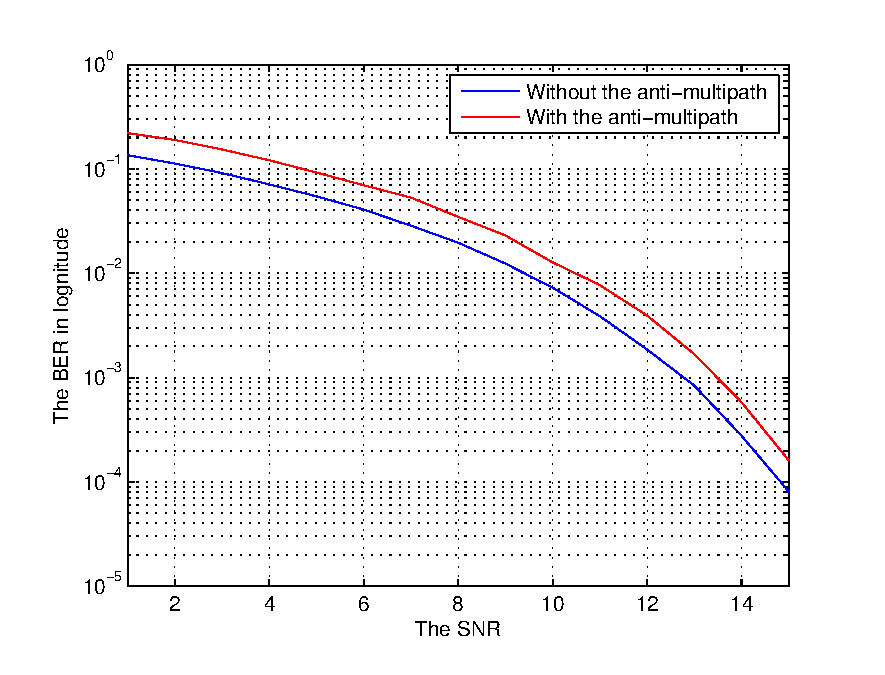
\includegraphics[width=0.8\linewidth]{6.eps}
		\caption{使用n=15重构误差波形及频谱}
\end{center}
\end{figure}
